\documentclass[]{marticle}
\usepackage{mstyle}

\graphicspath{ {./imgs/} }

\title{\textbf{\huge Predicting and Explaining on Electronic Health Records with Transformer-based Models}}
\date{}

\newcommand{\ds}{\mathcal{D}}
\newcommand{\codes}{\mathcal{C}}
\newcommand{\codesin}{\mathcal{C}_\text{in}}
\newcommand{\tree }{\mathcal{T}}
\newcommand{\patients}{\mathcal{P}}
\newcommand{\visits}{\mathcal{V}}

\DeclareMathOperator{\Red}{Red}
\DeclareMathOperator{\FI}{FI}

\begin{document}
\maketitle
\newpage

\tableofcontents
\newpage

\section{Introduction}

Rapid growth of information systems in the healthcare sector has made large amounts of relevant data
available in the last decades. One very important and rich form of this kind of data is the
Electronic Health Records (EHR), among which we can find sequences of visit descriptions taken at
irregular time distances. Visits can consist in informations on the medical conditions, symptoms,
diagnoses, medications and actions taken during the admission. 

With large amounts of data available, a significant opportunity for the advancement of the quality of
the services offered is presented through its analysis. One important task is the prediction of
future analysis given the patient history in the form of EHR. This is a nontrivial task given the
high dimensionality of the problem and its temporal dependencies. However several approaches in the
field of deep learning have been proposed to tackle this task, mainly based on recurrent
architectures \deb{citazioni} while an exploration transformer-based architectures has just started
\deb{altre citazioni}.

Good predictive models are not enough though. Models as critical as those in the healthcare sphere
have to work in tandem with professionals. To increase the trustworthiness of the models,
predictions should not only accurate but also understandable by humans. However, inner logic of
state-of the-art deep-learning models is still poorly understood. Work has been conducted in the
last years to work around this limit, an important example being doctorXAI \cite{panigutti-xai}, an
agnostic explainable model specifically built to leverage ontological information. Its core idea is
to approximate the local behaviour of a opaque model with an intrisically explainable predictor.

In this thesis we want to improve and fully understand the capabilities of doctorXAI. Our aim is to
improve the predictive accuracy of the underlying model and to provide more insight into the
explanations provided by doctorXAI, to improve its usability and effectiveness for physicians. Thus
we work in several directions.
\begin{enumerate}
\item \emph{On learning a black box model:} We substitute the underlying recurrent black-box model
with a transformer-based one, trained on an updated version of the dataset. This allows for better
performances in the predictions.

\item \emph{On generating explanations:}  We propose a new method for generating a synthetic
neighborhood that should be aware of the underlying data distribution. This would allow for a more
thorough exploration of the local behavior of the predictive model. The process would be done by
adding noise to real data and then extracting samples over a distribution for the possible
reconstruction given by a deep learning model.

\item \emph{On explaining:} We try to explore some parts of the transformer black-box model
through the lens of the local explanation. In particular, we will notice some correlation between the
attention score given by the self-attention heads in the transformer and the feature importance
given by the tree in the local explanation pipeline.
\end{enumerate}

\section{Related}


\subsection{LLM and Transformers}

The development of predictor models for categorical sequential data has historically been deeply
intertwined with text generation and machine-translation tasks. In the most common approaches,
the text is divided into smaller portions called tokens, which usually represent a word, a suffix, a
punctuation symbol, or an indivisible part of the language. Typical values for the number
of tokens in a single language are in the order of a few tens of thousands.

The text generation task is the problem of generating a text answer to a text prompt, which can be a
question or some kind of instruction. The machine translation task is the problem of generating the
translation to some given input text. These two tasks are very similar, and for clarity, we will
focus on the translation one  in the following discussion.

Handling sequence of data of arbitrary length has always been a challenge in the context of deep
learning, due to the fixed size of the input and output layers in Neural Networks. The first
effective solution has been the idea of recurrent architectures.

The task is split in two parts: in the first part the model gets in input the tokens of the prompt
to translate. In the second part the answer is generated in an autoregressive manner: starting from
a special \c{<start>} token, the model generates the next token. The new token is then concatenated to
the previous ones, and is given to the model, which generates a next token. This process continues
until a special \c{<end>} token is generated, or the generated sequence length exceeds a fixed limit.

\subsubsection{Recurrent Models and Attention}

A recurrent model is built in such a way that it can take in input a hidden memory vector $h$, and a
token $t$, and then outputs $h'$, an updated version of $h$. The new hidden vector is then fed to
the model together with the next token.

The process is started with a fixed initial vector $h_0$, and let's assume the prompt is made by the
token sequence $t_0, \dots, t_n$. Then given the recurrent model $f$, the first hidden vector
generated is $h_1 = f(h_0, t_0)$, and in general we define $h_(i+i) = f(h_i, t_i)$ for $i=1\dots n$.
This tackles the first part of the problem. 

A very simple form for the model $f$ is the following. Let $e_1, \dots, e_N$ be a sequence of fixed
$k$-dimensional vectors (these are called embeddings), where $N$ is the number of possible tokens
and $k$ is a fixed integer. Let $sigma$ be a non linear activation function, typical choices are the
Rectified Linear Unit (ReLU) or the sigmoid function. Let $W_h$ and $W_t$ be two $n \times n$
matrices a $b$ a $k$-dimensional vector. Then if $h$ is a $k$-dimensional hidden state, and $t$ a
token corresponding to the vector $e_j$, we set $f(h,t) = \sigma(W_h h + W_t e_j + b)$.

Other more complex architectures has been explored, but this simple presented one is the base for
all of them.

For the second part we start with a the \c{<start>} token which we will call $g_0$. From this we
generate a new hidden state $\hat{h}_1 = f(h_{n+1}, g_0)$. With a classical NN model $f_\text{gen}$ we can
use $\hat{h}_1$ to generate a probability distribution $f_\text{gen} (\hat{h}_1)$ over all the possible
tokens. We can then extract a new token from this distribution. Usual approaches consists in taking
the maximum probability token, a plain sampling over the distribution, or some hybrid methods in
which the sample is performed only on the most probable tokens. The result of this process is a new
token $g_1$. From this point onward we repeat the process, generating $\hat{h}_2 = f(\hat{h}_1, g_1)$
and from the new hidden state a new token, and so on.

The training of this kind of models is performed noticing that it defines a probability distribution
over all the possible answer sentences. In fact each new token is generated from a probability
distribution given the previous ones. This is effectively a decomposition of the probability of the
whole sentence. Thus the training is performed maximizing the likelihood of a dataset of human
generated pairs of input and outputs.

\begin{figure}[!h] 
\begin{center}
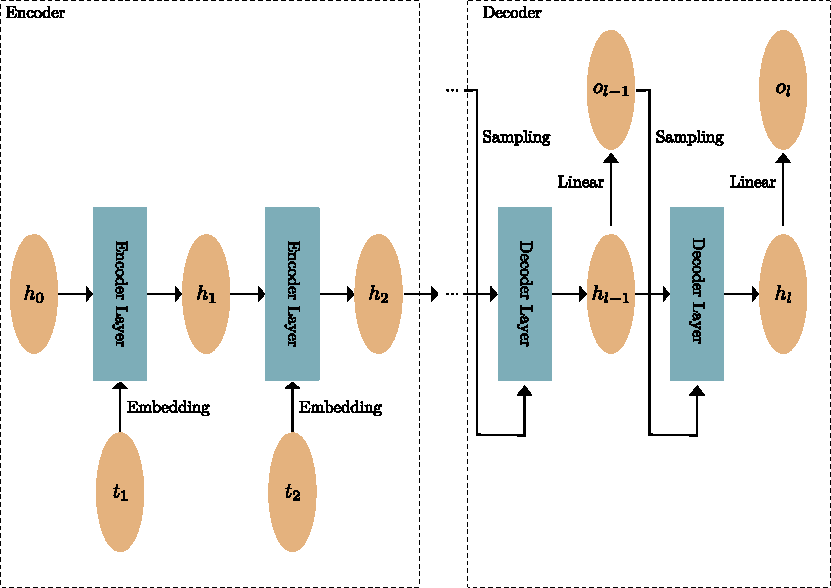
\includegraphics{recurrent_simple.pdf}
\caption{\deb{Recurrent architecture, simple.}} 
% \label{fig:your image label} 
\end{center}
\end{figure}

\begin{figure}[!h] 
\begin{center}
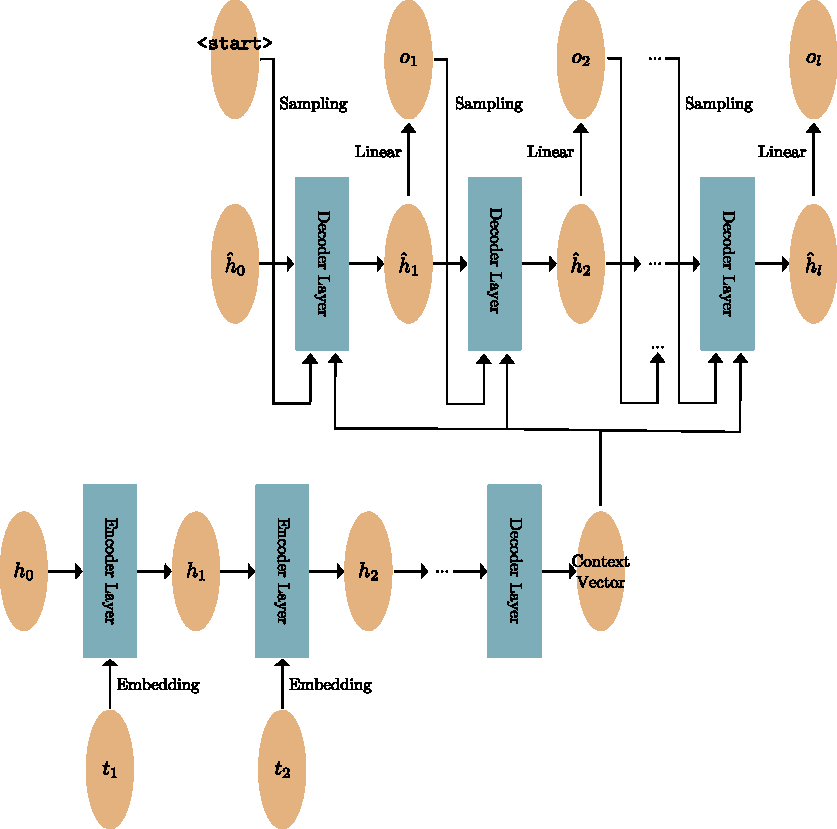
\includegraphics{recurrent_context.pdf}
\caption{\deb{Recurrent architecture, with context.}} 
% \label{fig:your image label} 
\end{center}
\end{figure}

\begin{figure}[!h] 
\begin{center}
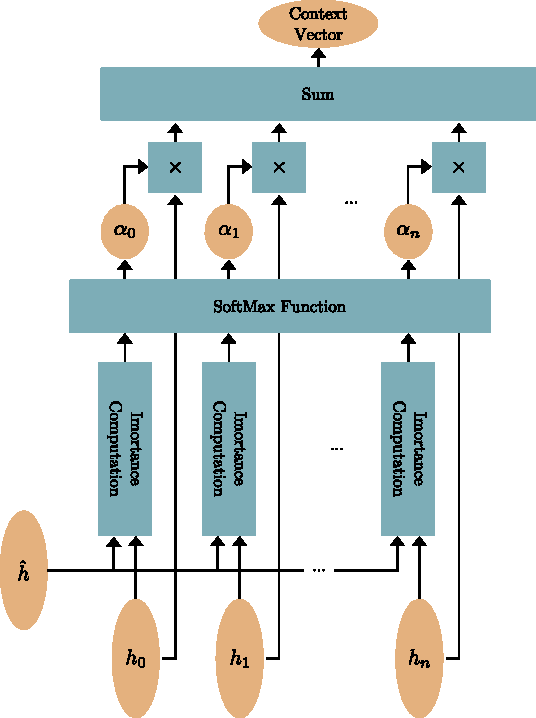
\includegraphics{context_with_attention.pdf}
\caption{\deb{This is how we compute the context with attention}} 
% \label{fig:your image label} 
\end{center}
\end{figure}

\begin{figure}[!h] 
\begin{center}
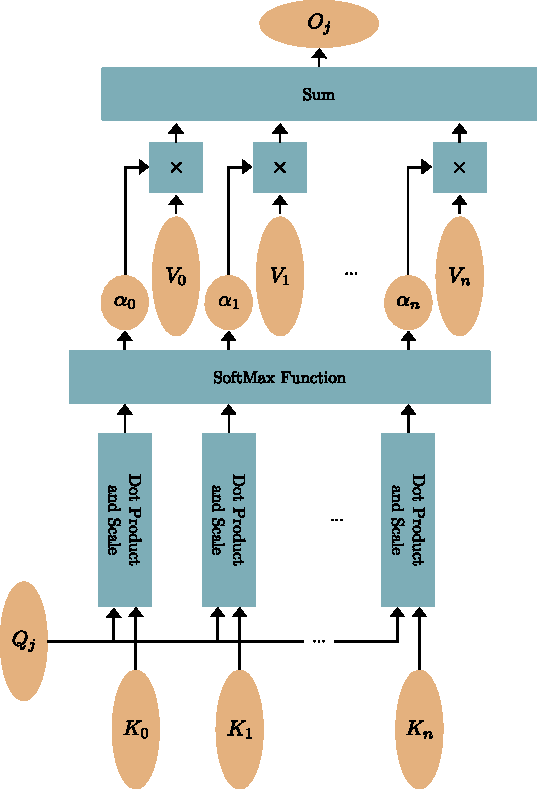
\includegraphics{self_attention_architecture.pdf}
\caption{\deb{This is the architecture of a self attention head. This structure is repeated for every index $j$}} 
% \label{fig:your image label} 
\end{center}
\end{figure}

\begin{figure}[!h] 
\begin{center}
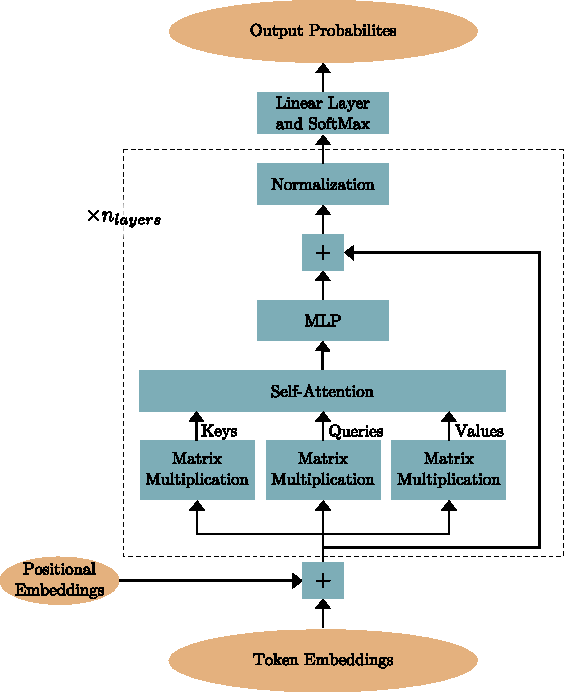
\includegraphics{transformer_architecture.pdf}
\caption{\deb{This is the architecture of a simple LLM.}} 
% \label{fig:your image label} 
\end{center}
\end{figure}

As in most of trainings of Neural Networks, the optimization is done through Stochastic Gradient
Descent and backpropagation. This reveals the biggest weakness of recurrent architectures. Assuming
the model has parsed $n$ tokens between inputs and outputs, which means that reasonable values for
$n$ could range from a few dozens to few hundreds or even more, the gradient for the first
application of $f$ has to go through all the $n$ layers that follows to arrive to the loss. During
all these steps the quality of the gradient is degraded, usually leading to the phenomenons of
exploding gradients or vanishing gradients. The idea is that the flow of the gradient is a dynamical
system which can be mostly described by a multiplication by a a matrix. If these matrices
consistently increase the magnitude of the gradient, the gradient will become very large, and thus a
step of SGD will move the model parameters in a region in which the function cannot be approximated
by the gradient in the starting point. This means that the update is meaningless. If instead the
matrices consistently decrease the magnitude of the gradient, the update of the SGD will be near
zero, and the model will fail to converge.

Several attempts to solve this problem have been tried by modifying the inner architecture of the
recurrent net, and the most notable examples of that are the Gate Recurrent Units (GRUs) and the
Long Short Term Memory models (LSTMs). These are however only a mitigation of the problem, and not a
complete solution.

One first possible modification, that does not solve the gradient problem but still improves the
performances of the model is using two different models for the two parts of the task. These two
models have the same structure of the previous recurrent ones, but they are used for two different
objectives. The first part of the problem is to encode the input tokens into a single hidden vector,
and thus the model is called encoder. The second part of the problem is to take the hidden vector
and generate autoregressively the output, in fact decoding the vector into tokens. This second model
is thus called decoder.

A very important step for the evolution of these architectures has been in noticing that the hidden
state during the decoder phase of the process has two distinct functions: remembering the input, and
remembering at which point of the output generation the model is at. This suggest that the two
functions could be carried out by two different vectors. This can be easily accomplished by having
the decoder model be a function of a decoder hidden state, a context vector, which is the final
output of the encoder, and the previous token. The result is that the decoder is unable to forget
the encoder output, because it is not modified during the recurrence.

The next step has been improving this mechanism. In the translation task, it's very common for a
word in the output to map directly to a single word in the input, and more generally small groups of
words in the outputs correspond to small groups of words in the input. On the other hand most of the
data produced by the encoder, the hidden states, is discarded, keeping only the last hidden state.
As a consequence an arbitrary large amount of data, the input tokens, has to be compressed in a
single hidden state, whose size is fixed by the model architecture. The following idea improves over
this direction.

Let's assume that the encoder has generated the hidden states $h_0, \dots, h_n$, and let $\hat{h}$ be
the current hidden state in the decoder. In the previous architecture we would need a fixed context
vector generated from the encoder. What we do now is to generate a context vector dependent on
$\hat{h}$. The first step is to have a measure of how important is a given hidden state $h_i$
according to $\hat{h}$. In the most simple version of the architecture, this measure is simply the
dot product $h_i^\top \hat{h}$, but other differentiable functions of the two vectors could be used.
Once the importances $x_0, ..., x_n$ are given, they are converted on a distribution probability
over the hidden vectors of the encoder. This is done through the SoftMax function:
$$ \alpha_i = \frac{\exp (x_i)}{\sum_j \exp (x_j)}. $$ 
The idea is that the probability distribution measures how relevant is each hidden state for the
current prediction, and thus how much attention should be given to each of them. The distribution is
in fact called attention. With this in mind, the context vector is simply the mean of the hiddden
states, weighted through the attention:
$$ c = \sum_i \alpha_i h_i. $$

This is very important because attention allows the gradient to ``take shortcuts'' to get to the first
layers without having to pass through all the following ones.

One important way to scale up in size and complexity all the previous models is to have several
layer the recurrent architectures. These leads to have a first layer similar to the ones described
before: it takes as an input the previous hidden state, the embedding of a token, and in some cases
a context vector. Each of the subsequent layers takes in input the previous hidden state for that
layer, the hidden state of the previous layer, and sometimes the context vector.

\subsubsection{Transformers}

The next iteration on these design led to the current State of the Art models like GPT-3.5 or Llama.
The idea is to get rid entirely of the recurrent part, focusing only on the attention. The heart of
these models is the transformer. It is a layer that takes as an input a set of $d$-dimensional
vectors $e_1,..., e_n$ and returns a set of vectors of the same size. By means of a multiplication
by some fixed matrices $W_k$, $W_q$ and $W_v$ of size $d\times d_h$ where $d_h$ is called hidden
size, the vectors $e_i$ are mapped to three sets of vectors: keys $K_i = W_k e_i$, queries $Q_i =
W_q e_i$ and values $V_i = W_v e_i$. The keys perform the same role of the hidden states $h_i$ when
choosing the importances in the previous discussion. The queries are the anologous of the vector
$\hat{h}$, while the values are the vectors that will be combined through a weighted average.

For each query vector, a measure of importance is computed as before as the dot product with each
key value. This result is often scaled by the square root of the number of dimensions $d_h$, which
while it does not improve the expressiveness of the model, it balance the fact that increasing $d_h$
is reflected in bigger dot products. These importances are then processed in a SoftMax function to
give the attention probability distribution:
$$ \alpha_i = \text{SoftMax}((Q_i^\top K_0, \dots, Q_i^\top K_n) / \sqrt{d_h}) $$
where 
$$ \text{SoftMax}(y_1,...,y_n)_i = \frac{\exp(y_i)}{\sum_j \exp (y_j)}. $$
The output is again obtained by means of a convex combination:
$$ O_i = \sum_j \alpha_{i,j} V_j $$

The previous relationships can be expressed in a more compact form seeing the vectors $K_i$, $Q_i$
and $V_i$ as column of the matrices $K$, $Q$ and $V$. Thus we obtain:
\begin{equation}\label{attn-ref}
O = \text{SoftMax} (Q K^\top/\sqrt{d_h})V
\end{equation}

Since the keys, queries and values are obtained from the same set of vectors $e_i$, the expression
\ref{attn-ref} is called self-attention head.

Usually more than a single self-attention head is present in a transformer layer. In an
$m$-headed transformer there are $m$ triples of matrices $W_k^{(i)}$, $W_q^{(i)}$ and $W_v^{(i)}$,
and each of them is used to compute the respective output $O^{(i)}$ for $i=1,..., m$. These outputs
are concatenated and brought back to the right dimension by means of a linear projection through a
matrix $W_o$ of size $m d_h\times d$:
$$ y = \text{Concat}(O^{(1)},..., O^{(m)}) W_o. $$

Multiple transformer layers can be stacked on top of each other. Since the only source of
non-linearity is the SoftMax function, which appears only in the coefficients of the values, vectors
usually go through a Feed Forward Network (FFN) between a transformer layer and the other. These
networks are usually very simple, often in the form
$$ \text{FFN}(y_i) = W_1 \sigma(W_2 y_1 + b) $$
where $\sigma$ is an activation function, usually a ReLU, and $W_1, W_2, b$ are parameters of
suitable size. This component is also called Multi-Layer Perceptron (MLP).

As in most deep learning models, skip connections and layer normalizations are also added.
\deb{Di più?}

In the recurrent models the order of the tokens was given to the model implicitely, because the
their embedding were fed in the right order. The same does not apply in transformer models: a
permutation of the inputs leads just to the same permutation on the outputs. In other words the
transformer cannot distinguish the order of the inputs by itself, and additional informations are
needed. While this can add to the complexity of the model, it also means Transformers are more
flexible by recurrent models.

The most common way to add temporal information is performed by adding to each input vector of the
transformer $x_i$ a fixed vector dependent by time only $p_i$. Thus while $x_i$ changes for each run
of the transformer, which will have different inputs, $p_i$ is fixed among all these runs. There are
different choices for $p_i$. One is to have it completely learnable by SGD. Another is to fix it,
usually to a vector in the following form:
$$ p = \begin{pmatrix}
\sin\omega^{1/d} i \\
\cos\omega^{1/d} i \\
\sin\omega^{2/d} i \\
\cos\omega^{2/d} i \\
\vdots \\
\sin\omega^{h/2d} i \\
\cos\omega^{h/2d} i
\end{pmatrix}
$$

where usually $\omega$ is taken to be 10,000.

This kind of vectors has showed to perform well. A possible line of reasoning for its justification
is that vectors of sines and cosines can be translated in time with just linear transformations,
which are easily performed within the model.

We observe that the length of the path between each output vector and each input embedding is not
dependent by the distance between the corresponding token, but they interact directly in the
attention computation. This completely solves the biggest issue of the recurrent models.

Another big advantage of transformer based models respect to recurrent ones is that all the
computations can be carried out in parallel, instead of having to find the hidden state of the
previous iteration in order to be able to start the next one. This allows a better usage of GPUs and
therefore smaller training times.

Moreover, in a training phase, all the outputs can be computed in one single sweep. This should be
done carefully though, because the prediction of the $i$-th cannot be performed by having as input
the $i+1$-th token, or even the $i$-th token itself. This can be done by tweaking the attention
matrices, imposing that the attention for the $i$-th query and the $j$-th key are zero whenever $i
\leq j$. The easiest way to accomplish this is by setting the corresponding importances to minus
infinity, which in turn will translate to zero through the SoftMax function. This correspond to add
to the importance matrices some upper triangular matrices.

Attention masks can be useful for another purpose as well. Until now we considered a single pair
input/output going through the model at each step of the training process. However usually deep
learning models are trained using minibatches of data for each step. This can be accomplished by
running multiple ``single pass'' steps, one for each element of the minibatch, and accumulating the
gradient. It may be more perfomant to deal with the minibatch in a single pass. This can be done by
concatenating all the data for the minibatch in a new dimension of the matrices, and the model
doesn't change much to accommodate this modification. However in general the sequence length will not
be constant through the minibatch. Thus all the sequences are padded to the max length within the
minibatch, and the attention mask is tweaked to avoid that any output depends on a padding token.

All of this tweaks allows the model to grow in size while still being trainable. In the last year in
fact there have been proposed several of such models, varying in size between a few billions
parameters to hundred of billions of parameters. These are called Large Language Models, or LLMs.
Examples are the GPT family developed by OpenAI, and the Llama family, developed by Meta.

\subsubsection{The Llama-2 Models}

The Llama-2 are a family of LLMs sharing the same underlying architecture and available in different
sizes: 7B, 13B, 34B and 70B, where the number counts the number of trainable parameters of the
model. The architecture is the same transformer-based decoder described in the previous section,
with the following modifications.
\begin{enumerate}
\item The normalization layers, used to prevent internal covariate shifts, are substituted with Root
Mean Square layer normalizations (RMSNorm) \cite{paper-rmsnorm}. The usual normalization layers
performs affine transformations on the hidden states such that the activations in a layer have mean
zero and standard deviation one. RMSNorm simply scales those activation such that the root mean
square is zero. This has showed to perform almost as better as the original version in terms of
loss, but is faster to compute.

\item The positional encoding have been replaced by Rotary Position Embeddings. The idea is to add
positional information at each layer of the model, modifying the key and query vectors by a
suitable function dependent by time. Let this modification be represented by the functions 
$f_k(y_n, n)$ and $f_q(y_n, n)$, where $y_n$ is the $n$-th vector of the previous layer or the
token embedding  multiplied by the matrix $W_k$ or $W_q$. Let's assume that the hidden dimension
to be an even number $d$, which is reasonable since for performance reasons typical values of
dimensions are large powers of two or some of their multiples. Then a good choice could be
$$ f_{\{q, k}\}(y_n, n) = R_{\Theta, n} y_m $$
where $R_(Theta, n)$ is a matrix in the following form:
$$
    R_{\Theta, n} = \begin{pmatrix} 
      R(n \theta_1)& 0& \dots& 0 \\
      0& R(n \theta_2)& \dots& 0 \\
      \vdots& \vdots& \ddots& \vdots \\
      0&0& \dots& R(n \theta_{d / 2})
    \end{pmatrix},
$$
$$
    R(\theta) = \begin{pmatrix} 
        \cos\theta & -\sin\theta \\ \sin\theta & \cos\theta
    \end{pmatrix},
$$
and $\Theta = \{ \theta_1, \dots, \theta_{d / 2} \}$ with $\theta_i = 10000^{-2(i-1) / d}$.

This choice has a nice property. Let $x_n$ and $x_m$ be the outputs of the previous layer. Then
the attention importance relative to the $n$-th query and $m$-th key using the Rotary Embedding
can be written as
\begin{align}\label{rotary-importance}
I_{n,m} &= (R_{\Theta, n}W_q x_n)^\top (R_{\Theta, m}W_k x_m) \\ 
        &=  x_n^\top W_q^\top R_{\Theta, m-n} W_k x_m. \nonumber
\end{align}
The matrix $R_{\Theta, m-n}$ is an orthogonal matrix, which helps the flowing of the gradient
during training. Moreover from equation \ref{rotary-importance} we can see that this is a kind of
relative encoding, which, in contrast with the absolute encoding, add informations only about the
distance of two tokens, and not their position in the whole sentence. For many tasks this is a
desirable property. One final remark is that the matrices $R_(Theta, n)$ are very sparse, and thus
the computation of the products can be performed in a $\Ocompl(d)$ complexity.

\item The MLP layers has been replaced with a Swish Gated Linear Unit (SwiGLU). The function Swish
is defined as
$$ \text{Swish}(x) = x \sigma(x) $$
where $\sigma$ is the sigmoid function. Given a hidden dimension of the model $d_h$ and a new
dimension $d_\text{MLP}$ for the MLP, we define the Gated Linear Unit as be parametrized by the
$W_\text{gate}$, $W_\text{up}$ and $W_\text{down}$, of size $d_h\times d_\text{MLP}$ for the first
two, and $d_\text{MLP} \times d_h$ for the last one. Let's denote the component-wise multiplication
of two vectors with the symbol $\odot$. Then the layer is defined as $$ \text{MLP}(x) =
W_\text{down} (\text{Swish}(W_\text{gate} x) \odot W_\text{up} x) $$ This approach has been proven
to have a better behaviour than a plain MLP layer.
\end{enumerate}

\subsection{Explainability}

New AI based on deep-learning techonologies show outstanding State-of-the-Art performances in many
fields. However, most of models based on deep-learning, random forests, or SVM are opaque, which
means that the inner reasoning that brought to the high accuracy results are not easy to extract
from the prediction.  Those models are then also called black-box models. Thus the last years
witnessed to an increasing interest in the field of eXplainable Artificial Intelligence (XAI), whose
objective is to augment the predictions with explanations understandable by humans.

Following the taxonomy of \cite{xai-survey}, we classify the most common XAI techniques as follows:

\begin{itemize}
\item Some models are \textit{explainable by design} or intrinsically explainable, which means that
    their reasoning behind each predictions is transparently available to the user. Examples are
    decision trees or linear regression models.

\item \textit{Post-hoc explanations} are those which complement an opaque black-box models, which is
    the source of the predictions. Examples are the methods that work in tandem with deep-learning
    models.
\end{itemize}

Focusing on the post-hoc methods, we categorize explanation algorithms on two distinct axis. The
first one describes what is being explained:
\begin{itemize}
\item \textit{Global} explainers try to explain the whole logic within the black-box model. The
    explanation is thus valid for each instance of the data.

\item \textit{Local} explainers on the other hand try to explain only a single prediction.
\end{itemize}

The second axis focus on the kind of information the explainer leverages on:
\begin{itemize}
\item \textit{Model-Specific} methods can use some data obtained from within the associated
    prediction model. Examples are the gradient from deep-learning models or attention values from
    transformer models.

\item \textit{Model-Agnostic} methods can only use the predictions given by the black-box. This
    means that any kind of black-box can be successfully used in tandem with this kind of
    explainers.
\end{itemize}

We proceed to show some important groups of explanation techniques.

\begin{itemize}

\item \textit{Prototypes}. The user is presented with data which may taken from a dataset or
    generated artificially, that gives examples similar to the input of the predictions that get a
    similar prediction.

\item \textit{Counterfactuals}. This method is similar to the prototypes, but work in the opposite
    direction: the counterfactuals are data similar to the input but with different prediction.

\item \textit{Feature importance}. This method is suited for tabular data, where each instance to be
    explained is a sequence of features $(x_1, x_2, \dots, x_n)$. The explanation consists in a
    vector $e=(e_1, e_2, \dots, e_n)$ where each component $e_i$ gives the importance of the
    corresponding feature $x_i$. Usually e positive value of $e_i$ can be interpreted as the feature
    $x_i$ contributing positively toward the given prediction, while negative values indicate that
    the feature contributes negatively.

\item \textit{Rule based}. The goal of this method is to find a set of rules that mimic the
    black-box at least on a subset of the data near the input to be explained. A rule consists in a
    boolean condition over the data and a prediction to be assigned when the condition is satisfied.

\item \deb{Ce ne vanno altre?}
\end{itemize}

\subsubsection{Decision Tree Classifiers}

An important example of intrinsically explainable models are the tree classifiers
\cite{tibsharani-elements}, \cite{trees-breiman}. Let $\ds=(x^{(1)}, x^{(2)}, \dots, x^{(k)})$ be a
dataset of $n$-dimensional vectors, and let $(y_1, y_2, \dots, y_k)$ be a sequence of labels from a
finite set $\codes$. A decision tree classifier is a description of iterative splits of the
$n$-dimensional space in partitions that contains data points $x_j$ with similar labels.

A decision tree classifier is a binary tree whose nodes are represented by a couple $i, t$ where $i$
is the index of a feature, so $i=1,\dots,n$, and $t\in\R$ is a threshold value. A subset of the
dataset is associated to each node of the tree: the whole dataset is associated to the root node,
and if the subset $D$ is associated to a non-leaf node $\theta = (i, t)$ then the subsets
\begin{align*}
    D_\text{left}  &= \{x \in D \ |\ x_i \leq t\} \\
    D_\text{right} &= \{x \in D \ |\ x_i >    t\}
\end{align*}
are associated to its left and right child respectively. We finally associate a label to each leaf
of the tree. Thus to each input $x$ the tree classifier predicts the label of the leaf associated to
$x$ through the rules.

One of the most common ways of finding a good decision tree is the CART algorithm
\cite{tibsharani-elements}. We first associate a number that measures the quality of the split in
each inner node.
\begin{equation*}
    G(\theta) = \frac{|D_\text{left}|}{|D|} H(D_\text{left}) + \frac{|D_\text{right}|}{|D|}
    H(D_\text{right})
\end{equation*}
where the function $H(D)$ returns the impurity of the set $D$. There are several options to choose
this function from, the most popular is the Gini index computed as 
\begin{equation*}
    H(D) = \sum_{j=1}^n p_j(D)\left(1-p_j(D)\right)
\end{equation*}
where
\begin{equation*}
    p_j(D) = \frac{1}{|D|}\sum_{(x,y)\in D}I(y = j)
\end{equation*}
and $I$ is the indicator function.

The tree is then built recursively and greedily, by assigning to each node the rule $\theta$ that
minimizes $G(\theta)$, until a maximum depth is reached. In a second phase of the algorithm, the
tree is pruned by removing nodes to reduce the complexity of the predictor.

To each non-leaf node we can associate an impurity reduction measure defined as 
\begin{equation*}
    \Red(\theta) = \frac{|D|}{|\ds|} \left( H(D) - \frac{|D_\text{left}|}{|D|}H(D_\text{left})  -
    \frac{|D_\text{right}|}{|D|}H(D_\text{right}) \right).
\end{equation*}

This measure describes how successful each node is in decreasing the impurity in a region. We can
use this impurity reduction to measure the impact of a feature on the decisions taken by the
classifier. Given a decision tree $T$ and a feature $j$, its importance $\FI(T, j)$ is the sum of
the impurity reduction over all inner nodes that split on the feature $j$. More formally if 
\begin{equation*}
    \Theta_j = \{(i, t) \in T \ |\ i = j\}
\end{equation*}
then 
\begin{equation*}
    \FI(T, j) = \sum_{\theta \in \Theta_j} \Red(\theta).
\end{equation*}

\section{Problem Description}

\subsection{Data Type} \label{sect-datashape}

Let $\codes$ be a finite set of discrete elements called codes. A visit is defined as any subset
of $\codes$. A patient is defined as a finite ordered sequence of visits. A code is allowed to
appear more than once within different visits of the same patient. Let $\visits$ be the set of all
possible visits, and $cal("P")$ be the set of all possible patient.

A dataset $\ds$ consists of a sequence of patients from $\patients$.

We assume that there exists a probability distribution $mu$ on the set $\patients$, which measures
the plausibility of each patient in a Bayesian sense, and we assume that $\ds$ is a sequence of
independent patients $p_1, \dots, p_N$ sampled from that distribution.

We can factor $\mu$ over each visit in the following way: let $p=(v_1, \dots, v_k)$ be a patient. Then
we decomposition is given by
$$ \mu(p) = \mu_0(v_1) \mu_\text{next} (v_2 | (v_1)) \mu_\text{next} (v_3 |
    (v_1, v_2)) \cdots \mu_\text{next} (v_k | (v_1, \dots, v_{k-1})) $$
where $\mu_0$ is a probability distribution over the initial visits $\visits$, and $\mu_\text{next}$ is a
probability distribution over the next visit given the preceding ones. In other words $\mu_\text{next} (v
| p')$ is the probability of $v$ being the next observed visit after seeing all the visits in $p'$.
\deb{Probabilmente ci dovrebbe essere una 'visita terminale' per dire quando la sequnza finisce.}

A predictor model $h(\cdot, \theta)$ parameterized by a vector of parameters $\theta \in \R^d$, for some
number of dimensions $d$, is a function
$$ h(\cdot, \theta) : \patients \arr [0,1]^{|\codes|}. $$
The underlying idea is for $h$ to be a predictor of the next visit for a given patient. In fact we
can see $h(p, \theta)$ as a distribution on the visits $\visits$, where we assume that each code is
chosen independently from each other, and the $i$-th code has a probability of appearing given by
the $i$-th component of $h(p, \theta)$. For example the vector $x=(x_1, \dots, x_{|\codes|})$ assigns
to the visit $v=(c_{i_1}, \dots, c_{i_n})$ the probability $\prod_j x_{i_j}$. In the following
discussion we will identify the vector $x$ with its distribution on $\visits$.

The objective of a training process is to find an optimal parameter $\hat{\theta}$ for which the
function $h(\cdot, \hat{\theta})$ is the best approximation of the distribution $\mu_\text{next}$. Since the
latter is never known, we will use the empirical distribution found in the dataset $\ds$ as its proxy.

\subsection{Ontology} \label{sect-ontology}

In many fields, and in particular the medical one, which is of our interest, some categorical data
is not just made of indistinguishable labels, but rather by leaf-nodes of a tree. This can be
formally described as follows. Let $\codesin$ be a set of ``inner nodes'', and let $\codes' = \codes
\cup \codesin$. Let $\tree$ be a tree with nodes $\codes'$ and whose leaves are all and only the
codes $\codes$. This tree is called ontology and gives some information over the codes in $\codes$
that appaeres in the dataset. We will assume that codes that are closer with respect to the distance
on the graph $\tree$ to be more similar than codes that are less close.

As done in \cite{panigutti-xai} we proceed to describe a distance on the possible patients $\patients$. To
do that, we will use a distance over the codes $\codes$ and the visits $\visits$.

We start describing a code-to-code distance. It is the Wu-Palmer similarity score, which is one of
the most commonly used for the ICD ontology. Let $c_1$ and $c_2$ be two codes in $\codes$. Let $L$
be their lowest common ancestor on the tree $\tree$, and let $R$ be the root of $\tree$. Let $d(c_1',
c_2')$ be the distance between codes in $\codes'$ which measures the smallest number of steps needed
to reach $c_2'$ starting from $c_1'$ and moving along the edges of the graph $\tree$. the Wu-Palmer
similarity score is then defined as
$$ \text{WuP}(c_1, c_2) = \frac{2 d(L,R)}{d(c_1,L) + d(c_2, L) + 2d(L,R)} $$

We observe that $0 \leq \text{WuP}(c_1, c_2) \leq 1$ for each pair of codes, and the minimum value $0$ is
reached when $L$ is the root of the tree, while the maximum value $1$ is reached when $c_1 = c_2 =
L$.

We can then define a visit-to-visit distance. The approach of \cite{panigutti-xai} is to use an edit
distance weighted through the Wu-Palmer similarity. However would need to choose an order between
the codes of each visit, while the codes do not have a natural order. For this reason we will follow
a different approach. Let $V_A = \{c^A_1, ..., c^A_a\}$ and $V_B = \{c^B_1,..., c^B_b\}$ be two visits
composed by $a$ and $b$ codes respectively. For each code in $V_A$ we choose the best similar code
in $V_B$. We them sum all of the distances between the best pairs to get an asymmetric distance:
$$ d^\visits _\text{asym} (V_A, V_B) = \sum_{i=1}^a \min_{j=1...b} \text{WuP}(v^A_i, v^B_j). $$
We can symmetrize the above expression taking the maximum of the two permutations:
$$ d^\visits  (V_A, V_B) = \max(d^\visits _\text{asym} (V_A, V_B), d^\visits _\text{asym} (V_B, V_A)). $$

Assuming to have precomputed a table with all the distance pairs $\text{WuP}(c_1, c_2)$, the computation
of $d^\visits (V_A, V_B)$ has a complexity of $\Ocompl(n^2)$, where $n$ is an upper limit on the
size of the visits.

Finally we are ready to describe a patient-to-patient distance $d^\patients$. We do that through
the Dynamic Time Warp (DTW) Algorithm. It gives a measure of similarity between two time series that can
differ in speed. The idea is to find associations between two elements of each series, in our
context they are visits of two patients, subject to the following constraints:
- Every element of the first sequence must be associated to an element of the first one;
- The first and the last elements of each sequence must be associated between them, but they not to
  be their only association.
- The associations must be monotonical: Let the $i$-th element of the first sequence is associated
  to the $j$-th element of the second one, and a similar things happens for the $i'$-th element in
  the first sequence and the $j'$-th element of the second one. Then $i<i'$ implies $j\leq j'$.
We can give a cost to each way of associating two series: it is the sum of the visit-to-visit
distances between each associated pair. The DTW similarity is then defined as the minimum cost
between all the associations that respect the previous conditions.

This optimization problem can be solved with a dynamic programming approach. Here it follows the
algorithm in pseudocode:
\deb{Spudoratamente preso da Wikipedia}
\begin{verbatim}
int DTWDistance(s: array [1..n], t: array [1..m]) {
    DTW := array [0..n, 0..m]
    
    for i := 0 to n
        for j := 0 to m
            DTW[i, j] := infinity
    DTW[0, 0] := 0
    
    for i := 1 to n
        for j := 1 to m
            cost := d(s[i], t[j])
            DTW[i, j] := cost + minimum(DTW[i-1, j  ],    // insertion
                                        DTW[i  , j-1],    // deletion
                                        DTW[i-1, j-1])    // match
    
    return DTW[n, m]
}
\end{verbatim}
\deb{Posso spiegare più in dettaglio qui}

It should be noted that the measure we have defined is not a distance in the sense of the metric
spaces, in fact it cannot guarantee the triangular inequality. Moreover if the number of visit per
patient is bounded by $m$ and the number of codes per visit is bounded by $n$, then there will be
$m^2$ iterations within the DTW algorithm, each of those will require a computation of the
visit-to-visit distance, which costs $\Ocompl(n^2)$ iterations. Thus the total cost of the
algorithm is $\Ocompl(m^2n^2)$.

\subsection{DoctorXAI} \label{sect-drxai}

DoctorXAI \cite{panigutti-xai} is a tool composed by two distinct parts. A predictor, called
doctorAI \cite{paper-doctor-ai}, and a novel explanation pipeline. \deb{Un capitolo a parte per
doctorAI?} For the explanation, given a patient history $p$, a neighborhood $N$ is generated. Then an
intrisically explainable predictor is trained on $N$. The final explanation is extracted from this
latter predictor.

\newcommand{\realds}{N_\text{real}}

Let $\ds$ be a dataset of real patients for explanation purposes. Let $d$ be the patient-to-patient
ontology-aware distance described in section \ref{sect-ontology}. We then extract from $\ds$ the $k$
patients that are the closest to $p$ according to $d$. This will form the real neighborhood
$\realds$ of $p$. The natural number $k$ is a parameter of the algorithm.

The following step is to augment $\realds$ with synthetic patients. In order to not introduce too
much noise into the final dataset $N$, synthetic patients are generated only through deletion from
real patients. The deletion is performed in an ontology-aware manner, as follows: given a patient
$p'\in \realds$, each code of its visits has a fixed probability $\theta\in [0,1]$ to be deleted. In
addition let $D=\{c_1, c_2, \dots, c_r\}$ be the set of such codes chosen for deletion. Let $c'_i$
be the parent of $c_i$ according to the ontology tree, for each $i=1,2,\dots,r$, and let $C'$ be the
sets of the $c'_i$ codes. Then the generated synthetic patient $p'$ is equal to $p$ when all the
codes whose parents appear in $C'$ have been deleted. We notice that for construction all the codes
in $D$ are deleted. In other words if a code is deleted, all the children of its parent are deleted
too.

We then need to associate a next visit prediction to each element of the neighborhood. This is done
by just running the black-box predictor on the data. A note on how the output is extracted should be
done. In fact the actual output of the black box predictor is a real number between zero and one for
each code, which defines the probability of that code to appear in the next visit according to the
predictor. Since these kind of predictors are evaluated with reacall at $k_\text{rec}$ metrics, the
predicted visit contains the $j$-th code when it is one of the first $k_\text{rec}$ most probable
codes. \deb{Non ho mai parlato di questa metrica prima.}

Since we are interested in explaing a specific prediction of a visit $v$, which thus contains
exactly $k_\text{rec}$ codes, we restrict the target labels through the whole dataset $N$ to those
codes. Therefore the target output has $k_\text{rec}$ dimensions.

We then have a dataset consisting in couples of patient history and prediction. The goal is to fit a
decision tree classifier on them, but unfortunatly one more step is needed to tackle the fact that
trees can only work on tabular data while we are dealing with complex data shapes. The proposed
solution is to encode all the codes in a single vector. Let $p=(v_1, v_2, \dots, v_n)$ be a patient
to be encoded. Each visit can be encoded in a fixed-size vector through a one hot encoding. If
$\codes$ is the set of all possible codes, the vector will have $|\codes|$ dimensions. Let
$\hat{v_i}$ be the codification of the visit $v_i$. Then
\begin{equation*}
    (\hat{v_i})_j = \begin{cases}
        1 &\text{if the $j$-th code appears in $\hat{v_i}$}  \\
        0 &\text{otherwise}.
    \end{cases}
\end{equation*}

Let $\lambda\in [0,1]$ be a fixed discount factor, parameter of the algorithm. In
\cite{panigutti-xai} a value of $\lambda = 1/2$ is used. Then we can aggregate the vectors
$\hat{v_i}$ with an exponential decay governed by the $\lambda$ factor. We thus obtain the final
encoding
\begin{equation*}
    \hat{p} = \sum_{i=1}^r \lambda^{r-i+1} v_i.
\end{equation*}

A tree is then fitted on this data, the inputs being $|\codes|$-dimensional real vectors and the
outputs being $k_\text{rec}$-dimensional vectors of zeros and ones. The explanation consists in the
branches taken by the patient to be explained $p$ when classifing it according to the trained tree.

Explanation are evaluated with three metrics:
\begin{enumerate}
\item Fidelity to the black box, which describes the perfomances of the tree predictions using the
black-box as the ground-truth. This metric is evaluated on a held-out set taken from the
neighborhood $N$. Since this is a multi-label classification task \cite{paper-multi-label}, a $F_1$
score with micro averaging.

\item A hit score, which measures how often the tree and the black-box models agree on the patient
to be explained. This is computed as the Hamming-distance between the two outputs.

\item A measure of complexity of the explanation. This is the depth of the leaf in the decision tree
corresponding to the patient to be explained, and represents the length of the explanation. This is
important because longer rules may be difficult to interpret by humans \cite{paper-lipton}.
\end{enumerate}

We can observe that there is a tradeoff to be done between the first two metrics and the third. In
fact deeper trees can lead to better agreements between the black-box and the explainable
classifier, but will lead to longer explanations.

\deb{We also notice that there is no metric available to understand how well the synthetic
neighborhood represents the data distribution...}
\subsection{Solution Proposal}

\section{Implementation of the Solution}

\subsection{Black-Box Model} \label{sect-kelso}

We build a new black-box model based on transformer architecture modyfing the Llama LLM \deb{cito il
mio capitolo o il paper?}. We observe that the shape of the data of a LLM is simpler than the one we
are dealing with. In fact text is defined in this context as a pure sequence of tokens, while our
medical data is a sequence of sets of labels, as described in section \ref{sect-datashape}. The
structure of our model is showed in Figure \ref{fig:kelso-architecture}.

\begin{figure}[!ht] 
\center
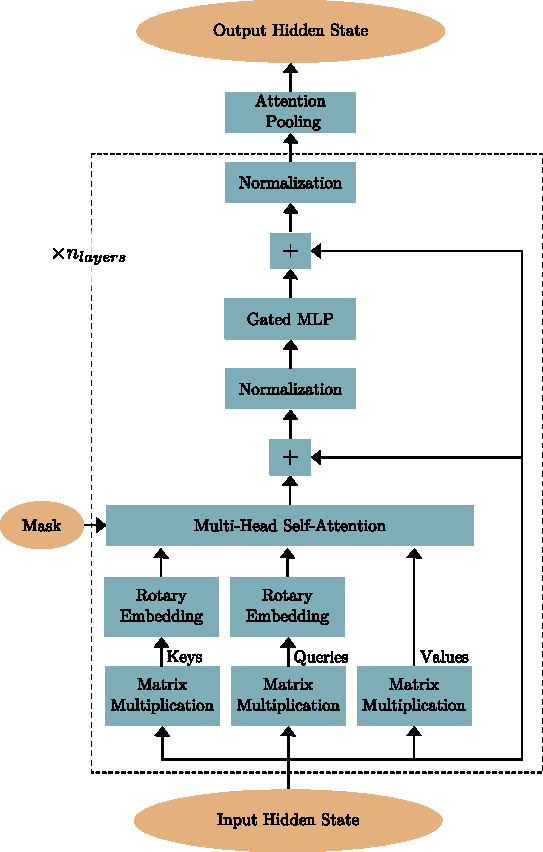
\includegraphics{kelso_architecture.pdf}
\caption{Architecture of the black box model.} 
\label{fig:kelso-architecture} 
\end{figure}

We will take advantage of the flexibility of the positional embeddings to pass the structure of the
data to the model. Let $p=(v_1, v_2, \dots, v_n)$ be a patient, where $v_i=\{c^{(i)}_1, c^{(i)}_2,
\dots, c^{(i)}_{m_i}\}$ are visits for $i=1,2,\dots, n$. Let $p'$ be the flattened sequence of codes
in $p$, in which the order within each visit is arbitrarily chosen:
\begin{equation*}
    p' = (c^{(1)}_1, c^{(1)}_2, \dots, c^{(1)}_{m_1}, c^{(2)}_1, \dots, c^{(2)}_{m_2}, c^{(3)}_1,
    \dots, c^{(n)}_{m_n}).
\end{equation*}

Then let $q$ be the sequence of natural numbers that specify the positional encoding, where $q_j$ is
equal to $r$ if $p'_j$ is a code corresponding to the $r$-th visit in $p$. We can then feed to the
transformer model the vector $p'$ to look up for the corresponding embeddings, one for each code,
and the vector $q$ to set the correct positional embedding. Since the positional embeddings are the
only part of the transformer where positions matters, the choice of the order of the codes when
forming the vector $p'$ does not affect the final result.

We notice that this could not be performed in a recurrent architecture, since permutations in the
order of the codes necessarily lead to different results.

Together with the tweaked positional embeddings a modification to the decoder mask should be done.
In fact keys and queries associated to codes within the same visit should be always allowed to
interact with each other. The mask should still prohibit codes in the future visits to ``look
into'' codes of previous visits. Thus the mask $M$ must have a block-wise triangular form, as
follows:
\begin{equation*}
    M_{i,j} = \begin{cases}
        0       & \text{when $q_i\leq q_j$} \\
        -\infty & \text{otherwise.}
    \end{cases}
\end{equation*}

At this stage the model is able to correctly handle the input data and its structure. However
transformers do not change the shape of the data, but while the input of the model has a length
equal to the number of the codes of the patient, the output should have a length equal to the number
of the visits. Since in general in the final layer of the transformer there will be a vector for
each code in $p'$, we adopt an additional layer to aggregate all the vectors regarding codes of the
same visit into a single one. This is called a pooling layer. We present two different versions of
it.

The simplest one performs a simple component wise average over the vectors to be aggregated. This
keeps the same ``consideration'' for each code in the visit, and has the nice properties to be
differentiable (which is needed for SGD), invariant under the permutations of the codes, and
the resulting vector does not have bigger magnitude for longer visits, as a sum would lead to.

\begin{figure}[!b] 
\center
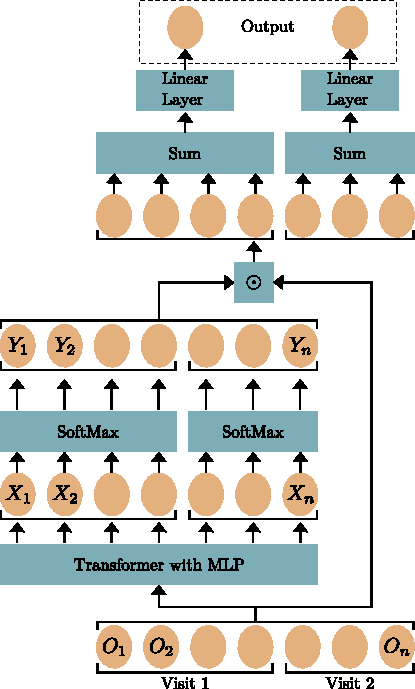
\includegraphics{attention_pooling.pdf}
\caption{Architecture of the Attention Pooling with parameters. This is an example with two vistis,
but it can be generalized to any number of visits.}
\label{fig:pooling-architecture} 
\end{figure}

The second version is parametrized, and allows for different codes to contribute in different
amounts to the visit vector. Its architecture is showed in Figure \ref{fig:pooling-architecture}.
Let $O$ be the output of the transformer, so it is a $m \times h$ matrix, where $m$ is the number of
the codes in the visit $m=\sum_i m_i$, and $h$ is the hidden dimension. We pass $O$ trough an
additional transformer layer to obtain a sort of ``importance'' matrix $X$. The transformer layer is
made up as usual by a multi-self-attention head and a MLP layer. Since the objective of this layer
is to pool together the codes in the same visit, the positional embeddings are disabled, and the
mask allows keys and queries vectors to interact only if they are relative to codes within the same
visit. More formally, the mask $M$ is defined as 
\begin{equation*}
    M_{i,j} = \begin{cases}
        0       & \text{when $q_i = q_j$} \\
        -\infty & \text{otherwise.}
    \end{cases}
\end{equation*}

We now have to act on $X$ such that we can define a probability vector over each visit. We do this
separately for each of the $h$ dimensions of the hidden vectors. As usual this conversion is done
with a SoftMax function. Let $Y$ the output of this operation and $j$ a selected column,
$j\in\{1,2,\dots h\}$. The matrix $Y$ will have the same shape of $X$. Let $i$ a selected row index,
$i\in \{1,2,\dots m\}$, such that the it corresponds to the $k$-th visit. Let $a$ and $b$ the index
of the first and last codes respectively in that visit. This means that 
\begin{equation*}
    a = \sum_{r < k} m_r + 1
\end{equation*}
and 
\begin{equation*}
    b = \sum_{r \leq k} m_r.
\end{equation*}

Then we define
\begin{equation*}
   Y_{[a:b], j} = \text{SoftMax}(X_{[a:b], j}),
\end{equation*}
where $Y_{[a:b], j}$ denotes the vector such that $(Y_{[a:b], j})_l = Y_{a+l-1, j}$ for ${{l=1,..., b-1}}$.

The resulting Matrix of the pooling is computed by summing all the vectors in $X\odot Y$
corresponding to each visit.

With both the versions of the pooling head, the output is a matrix of shape $n \times h$ where $n$
is the number of visits. A simple linear layer will be enough to bring the output at a shape equals
to $n \times |\codes|$ that represent the logits for the presence of each codes in the prediction.

Of course only the last vector will be used for inference, but the whole matrix is needed for the
training.

Another modification over the original Llama model is that we use the standard normalization layer
instead of RMSNorm. We make this choice because training times are not very long with the amount of
data we have.

\deb{Questa parte va in Experiments?}
A note on which codes are used should be made. Following the idea of other similar models
\cite{setor-paper}, we use ICD codes as inputs and CCS codes as output. This allows us to have more
accurate predictions than the case in which we used only CCS codes, while we keep a reasnable sized
output dimension.

This model is trained with an Adam algorithm with Decoupled Weight Decay Regularization
\cite{paper-adamw}. For each visit to be predicted the loss is computed as the code-by-code binary
cross-entropy. This is then summed over the codes and averaged over all the visits of the minibatch.

We performed a hyperparameter selection with a complete search running the candidate models for a
fixed amount of epochs, and choosing the best on the metrics obtained on a held-out validation set
of the data.

The final model is then trained until the metrics on the validation set stop getting better. The
model is then evaluated on another held-out test set.

\subsection{Generative Explanation Pipeline}

Our second proposal is about the generation of the synthetic neighborhood for the explanation
pipeline. We start as in section \ref{sect-drxai} with a real neighborhood $\realds$ of patients
selected to be as close as possible to the patient to be explained $p$. The notion of ``closeness''
is again formalized by the ontology-aware visit-to-visit distance of section \ref{sect-ontology}.
We can also perform generative perturbations on a dataset of synthetic patients generated with
ontological perturbations.

The ontology pipeline modifies the real patients only by deletion, to avoid introducing noise into
the neighborhood. That would mean having to run the black-box model on patients out of the original
distribution of the data. Our goal is to find a way to explore the neighborhood of $p$ by augmenting
the the real neighbors with new codes that are plausible. The idea is to have a model that codifies
the distribution of the data, and let the generative process be guided by that model.

\deb{Ispirazione da stable diffusion?}

We build a model that is able to reconstruct the original patients from noisy ones. Given a real
patient $p_r$, the noise is added by masking some randomly chosen codes present in their visit with
a special code \c{hole}. The input has thus the same shape as described in section \ref{sect-kelso},
but the codes vector is able to contain the new special code.

The model is then composed by the following stack of layers:
\begin{enumerate}
\item An embedding layer that associates each code to a $h$-dimensional vector. It can accept
$|\codes|+1$ distinct codes.

\item Several transformer layers. These are built in the same way as in section \ref{sect-kelso},
with all the care needed to encode the correct structure of the data through the positional
embeddings and the decoder masks.

\item An output layer which is a simple linear function that shifts the dimension of the data from
$n \times h$, which is the output of the transformer, to $n \times |\codes|$.

\item A final SoftMax function, which converts the logits of the output layer into vector of
probability over the codes.
\end{enumerate}

The procedure for generating a synthetic patient from a real one $p_r$ is done as follows:
\begin{enumerate}
\item The codes of $p_r$ are converted to their flattened form, and a vector of positional encodings
$q$ is built during the process.

\item Some codes chosen at random in the flattened patient are substituted with the \c{hole} code.

\item The noisy patient is fed to the generative model. For each code in input we have a
distribution of probability over the possible codes that can be placed in that position. We expect
this probability to be near a deterministic identity function when restricted to the unmasked codes,
and to reconstruct the original patients when restricted to the \c{hole} codes. \deb{???}

\item New codes are sampled from the distributions corresponding to the \c{hole} codes. The sampled
elements will substitute the \c{hole}s to obtain the final generated patient.
\end{enumerate}

\deb{Questa parte va in Experiments?}
The generative model must have ICD codes as outputs in order to be compatible with the black-box
model. To keep the output layer at a reasonable dimension we set the target codes to be slightly
different by the original patinet to be reconstructed: we masked all the codes that are not between
the $k_\text{out}$ most frequent codes in the dataset with a special ``\c{other}'' code. The outputs
sampled to be ``\c{other}'' are then left blank in the final generated patient.

For the training we selected two distinct possible losses to use: a multi-label categorical
cross-entropy over all the codes $l_\text{all}$, masked or not, and a similar multi-label
categorical cross-entropy computed only on the masked codes $l_\text{masked}$. Thus the final loss we
used is a combination of the two through an hyperparameter $\lambda _\text{loss}$:
$$ \text{Loss} = l_\text{all} + \lambda_\text{loss} l_\text{masked}. $$

The training is performed as in the black-box model using the AdamW algorithm.

\section{Experiments}

\subsection{Mimic IV}

Mimic IV \cite{mimic-iv-cit} is a dataset contaning medical informations resulted from the collaboration
of the Beth Israeli Deaconess Medical Center (BIDMC) and the Massachusetts Institute of Technology
(MIT). Data is gathered as part of the routine activities at BIDMC, and processed at MIT.

The dataset contains informations about patients accessing the services at the emergency department
or Intensive Care Units (ICUs) between 2008 and 2019. Patients that were below age 18 at ther first
admission time were excluded. People known to require extra protection were excluded as well.
Between the raw data sources and the final published dataset, a step of deintefication of the
patients has been performed, removing all personal informations and translating by a random time all
the events regarding every single patient.

The dataset is divided into three separate modules: \c{hosp}, \c{icu}, and \c{note}.

The \c{hosp} module stores information regarding patient transfers, billed events, medication
prescription, medication administration, laboratory values, microbiology measurements, and provider
orders. This is the main source of data of this project.

The \c{icu} module contains all the information collected by the MetaVision clinical information
system for the ICU units.

The \c{note} module contains textual data of discharges, which gathers an in-depth summary of the
patients history during their stays at the hospital, and a section about radiology data.

Our main interest is in the \c{hosp} module, which contains among other things a table of admissions
and a table of diagnoses. The admissions is a table that associates a patient id, an admission id,
several temporal coordinates for the admissions such as the admission, registration and discharge
times. There are also information about the patient like language, insurance, race and marital
status. We will use only the patient and admission id, and the relative ordering given by the
admission time. This table contains 431,231 rows, each corresponding to a unique admission. 

The diagnoses table is much larger, containing 4,756,326 rows, each with a unique diagnose. A
diagnose is composed by a patient id and admission id, which correspond to the ones given in the
admission table, a couple icd-version and icd-code, and a numerical priority ranging 1-39 which
ranks the importance of the codes within the same visit.

ICD, the International Classification of Diseases, which is a system to classify diagnostic
statements maintained by the World Health Organization (WHO). There are several versions of these
codes, and Mimic-iv uses ICD-9 and ICD-10. The version is flagged in a specific column of the
diagnoses table. A code may indicate signs, symptoms, abnormal findings, complaints, social
circumstances, and external causes of injury or disease. In Table \ref{table:icd_examples} are
reported some examples of ICD-10 codes. ICD-9 codes are very similar.

\begin{table}[h]
\begin{center}
\begin{tabular}{  c  l  }
    \hline
    \myalign{c}{Code} & \myalign{c}{Description} \\ 
    \hline
    A00.0 & Cholera due to Vibrio cholerae 01, biovar cholerae \\ 
    E66.0 & Obesity due to excess calories \\ 
    I22.0 & Subsequent myocardial infarction of anterior wall \\ 
    F32.0 & Mild depressive episode \\ 
    O80.0 & Spontaneous vertex delivery \\ 
    S81.0 & Open wound of knee \\ 
    W58   & Bitten or struck by crocodile or alligator \\ 
    Z56.3 & Stressful work schedule \\ 
    Z72.0 & Tobacco use (Excl. tobacco dependence) \\ 
    \hline
\end{tabular}
\caption{Some examples of ICD-10 diagnoses codes from different sections.}
\label{table:icd_examples}
\end{center}
\end{table}

In the diagnoses table of the Mimic-iv dataset there are 2,766,877 ICD-9 codes (58\% of the total)
and 1,989,449 codes (42\% of the total). Considering codes with different versions of ICD
categorization as different, the dataset contains 25,829 distinct codes, which means that each code
appears on average 184 times in the database. Of course the codes are not evenly distributed among
those present. \deb{Grafico della distribuzione}.


The admission table contains 180,733 distinct patients. However there are 101,198 patients (56\% of
the total) who are present in a single admission. We will filter those out because to make a
prediction that can be compared with a ground truth at least two visits are necessary. A percentage
of 92\% of patients has no more than five visits.

A preprocess phase is done by deleting all the patients who have a single visit, and then a
conversion from ICD-10 to ICD-9 is performed, such that all the models will work on a single
ontology. The data that follows will be referred to the subset of patients with at least two visits
in the dataset.

The conversion between the two versions of the codification is not straightforward, and some ICD-10
codes can be mapped to more than a ICD-9 code. Moreover, the conversion table we used \deb{quale?}
does not contain all the ICD-10 codes present in Mimic-iv. These are the 0.8\% of all the codes, and
are assigned to a special ``not found'' class. When multiple conversions were available we chose a
random one, as done in \cite{setor-paper}.

We convert the ICD codes to another system called CCS. \deb{qui non trovo il paper, e in effetti
tutti i paper che lo usano linkano solo al sito web...}

\subsection{Black-Box Model}

Before training the final model, we performed a hyperparameter tune algorithm over the following
hyperparameters:
\begin{itemize}
\item \textit{Hidden size}. This is the hidden size of the transformer, which is also equal to the
    size of the embedding vectors.

\item \textit{Number of layers}. It is the number of transformer layers present in the model.

\item \textit{Number of attention heads}. Number of self-attention heads in the transformer.

\item \textit{Attention head size}. This is the size of each key, query and value vector within each
    single self-attention head.

\item \textit{Learning rate}. This regulates the step size of the SGD algorithm.

\item \textit{Intermediate size of MLPs}, which is the size of the projection in the gated MLPs of
    the model

\item \textit{Parametrized pooling head}. It is a boolean value, which indicates whether to use the
    parametrized pooling head (when true), or the uniform one (when false).
\end{itemize}

We ran a complete hyperparameter search for choosing the best model, using the search space showed
in Table \ref{tab:hyper-kelso}. The search was performed by training each candidate model for 20
epochs, then we chose the model that showed the minimum loss on the evaluation set. \deb{The performance
of the models are not heavily influnced by the choice of hyperparameters if they have enough
trainable parameters. Most of the runs gave very similar results in facts.}

\begin{table}[h]
\begin{center}
\begin{tabular}{  c  l  }
    \hline
    \myalign{c}{hyperparameter} & \myalign{c}{Values} \\ 
    \hline
    Hidden size               & 63, \textbf{128}, 256        \\
    Number of layers          & 1, \textbf{5}, 10            \\
    Number of attention heads & \textbf{4}, 8                \\
    Attention head size       & 15, \textbf{32}, 64          \\
    Learning rate             & $\mathbf{9^{-3}}$, $10^{-4}$ \\
    Intermediate size of MLPs & 255, 512, \textbf{1024}      \\
    Parametrized pooling head & \textbf{True}, False         \\
    \hline
\end{tabular}
\caption{hyperparameter search space for the black-box model. The selected parameters are showed in
bold-face.}
\label{tab:hyper-kelso}
\end{center}
\end{table}

We trained the final model until the loss on the evaluation set stopped improving. The history of
the loss over the evaluation set is showed in Figure \ref{fig:kelso-train-loss}. We also kept track
of the recall metrics over the first 5, 10, 20 and 30 codes. The history of these metrics is showed
in Figure \ref{fig:kelso-train-recall}. The results show that our model performs better than the
version of doctorAI used in \cite{panigutti-xai}, but it still does not reach the performances of
more complex models as SETOR \cite{setor-paper}, which also uses the ontology for the predictions.
However one of the strengths of our model is its semplicity, which will allow us to perform the
analysis described in the next sections. Table \ref{tab:predictor-compare} compares the performances
of these three different models.

\begin{figure}[!tb] 
\makebox[\textwidth][c]{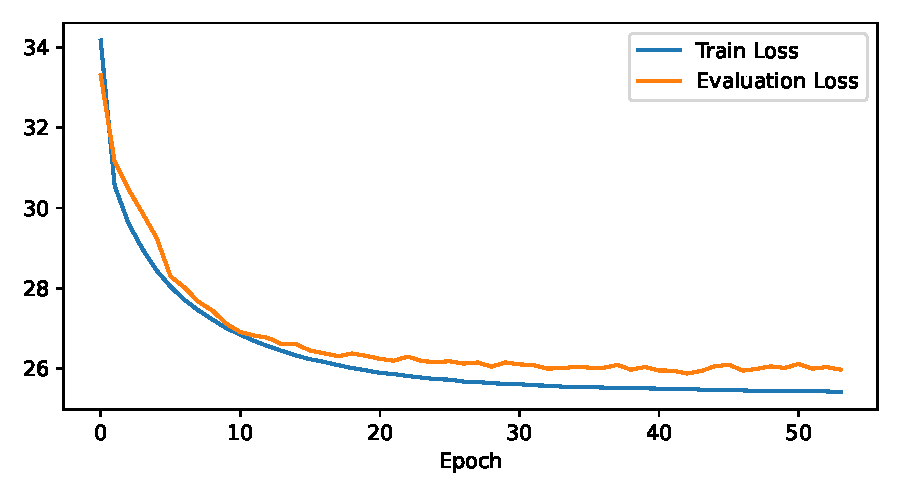
\includegraphics{kelso-train-loss.pdf}}
\caption{Loss history during the training of the predictor model.} 
\label{fig:kelso-train-loss} 
\end{figure}

\begin{figure}[!tb] 
\makebox[\textwidth][c]{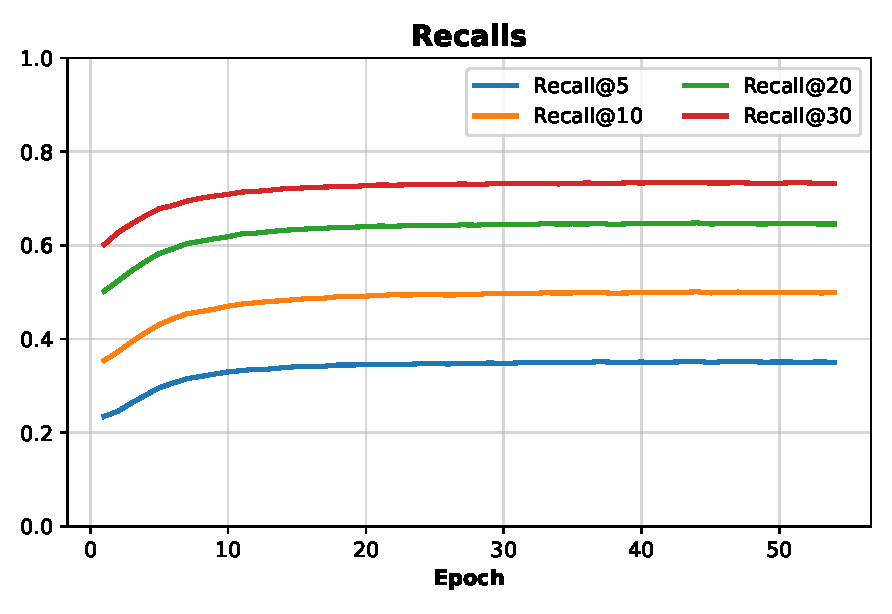
\includegraphics{kelso-train-recall.pdf}}
\caption{Recalls history during the training of the predictor model.}
\label{fig:kelso-train-recall} 
\end{figure}

\begin{table}[h]
\begin{center}
\begin{tabular}{  lccc  }
    \hline
    \myalign{c}{Model} & \myalign{c}{Recall@10} & \myalign{c}{Recall@20} & \myalign{c}{Recall@30} \\ 
    \hline
    doctorAI  & 35.0\% & 52.1\% & 63.1\% \\
    Our model & 50.8\% & 65.3\% & 73.7\% \\
    SETOR     & 70.6\% & 84.1\% & 88.2\% \\
    \hline
\end{tabular}
\caption{
    Comparison of the perfomances of different models.
}
\label{tab:predictor-compare}
\end{center}
\end{table}


We tried also training the model over a portion of the training set, while keeping the evaluation
and tests set at their original sizes. Figure \ref{fig:kelso-partial-train} shows the evaluation
loss and recall metrics as a function of the size of the training set.

\begin{figure}[!tb] 
\makebox[\textwidth][c]{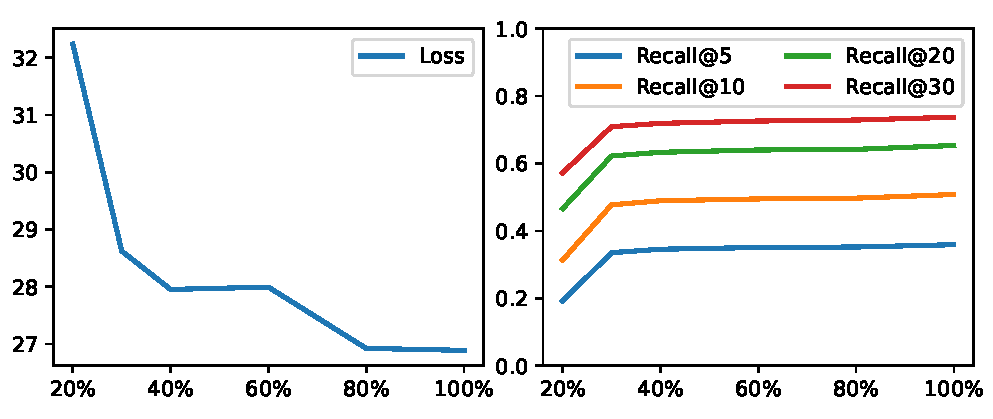
\includegraphics{kelso-partial-train.pdf}}
\caption{Metrics on the test set for the model trained on partial data. The percentage on the x-axis
indicates the portion of the train set used. \deb{Titoli etc..}}
\label{fig:kelso-partial-train} 
\end{figure}

\subsection{Explanation Pipeline}

We run the experiments on the explanation pipeline. Using the same hyperparameters of the predictor
model, we train a generator model on the train set. We set the number of possible output codes
$k_\text{out}$ to 500. The codes to be replace with \c{hole} are chosen independently with
probability $p_\text{hole}$. We tried values of $p_\text{hole}$ to $0.15$ and $0.25$, obtaining
similar results.

We generated the synthetic neighborhoods from the real neighborhoods in five distinct ways. The
first is the ontological perturbation described in \cite{panigutti-xai}. Then we used the generative
perturbations with two different methods, one guided by the generative model, and one with the new
codes sampled uniformely. Finally we used a combination of the two, running the generative
perturbation on top of the perturbations generated by the ontological pipeline.

Across the various combinations we kept the size of the synthetic neighborhood fixed at 32,000
patients. In the case of a single type of perturbation (ontological or generative) we generated
$n_\text{single}$ artificial patient from each real one. In the case in which we used both types of
perturbations, we generated $n_\text{ont}$ synthetic patients from each real one, and then
$n_\text{gen}$ patients from each on of the previously generated. Table
\ref{tab:multiplications-neigh} shows the multiplication factors we used for each size of the real
neighborhood. We notice that in some cases in the mixed generative method there are some unbalances
between $n_\text{ont}$ and $n_\text{gen}$, where we always favored the generative part giving it
more weight in the perturbation. We'll show however that despite this unbalance the results for the
mixed generation methods are more similar to the ones obtained from the purely ontological
perturbation.

\begin{table}[!h]
\begin{center}
\begin{tabular}{ cccc }
    \hline
      \myalign{c}{Real neighborhood size}
    & \myalign{c}{$n_\text{single}$}
    & \myalign{c}{$n_\text{ont}$}
    & \myalign{c}{$n_\text{gen}$} \\
    \hline
    100 & 32 & 4 & 8 \\
    200 & 16 & 4 & 4 \\
    400 &  8 & 2 & 4 \\
    800 &  4 & 2 & 2 \\
    \hline
\end{tabular}
\caption{
    Number of synthetic patients generated from each original real patient.
}
\label{tab:multiplications-neigh}
\end{center}
\end{table}


\begin{table}[!tb]
\begin{center}
\begin{tabular}{  cccccccc  }
    \hline
      \myalign{c}{Neighs}
    & \myalign{c}{Ont.}
    & \myalign{c}{Gen.}
    & \myalign{c}{Uni.}
    & \myalign{c}{Fidelity}
    & \myalign{c}{Corr/Max}
    & \myalign{c}{Corr/Min}
    & \myalign{c}{Corr/Avg} \\
    \hline
100 & Yes & No  & No  & 80.2\% & 0.30 & -0.08 & 0.03  \\
100 & No  & Yes & No  & 81.5\% & 0.23 & -0.04 & 0.04  \\
100 & No  & Yes & Yes & 81.7\% & 0.23 & -0.06 & 0.04  \\
100 & Yes & Yes & No  & 79.8\% & 0.27 & -0.11 & 0.02  \\
100 & Yes & Yes & Yes & 79.8\% & 0.28 & -0.07 & 0.03  \\
\\
200 & Yes & No  & No  & 80.1\% & 0.30 & -0.10 & 0.03  \\
200 & No  & Yes & No  & 81.6\% & 0.27 & -0.06 & 0.04  \\
200 & No  & Yes & Yes & 81.7\% & 0.26 & -0.06 & 0.04  \\
200 & Yes & Yes & No  & 79.9\% & 0.28 & -0.09 & 0.01  \\
200 & Yes & Yes & Yes & 79.9\% & 0.29 & -0.09 & 0.03  \\
\\
400 & Yes & No  & No  & 79.5\% & 0.28 & -0.10 & -0.00  \\
400 & No  & Yes & No  & 81.3\% & 0.27 & -0.10 & 0.02  \\
400 & No  & Yes & Yes & 81.4\% & 0.29 & -0.07 & 0.03  \\
400 & Yes & Yes & No  & 79.4\% & 0.27 & -0.13 & 0.00  \\
400 & Yes & Yes & Yes & 79.4\% & 0.26 & -0.10 & -0.01  \\
\\
800 & Yes & No  & No  & 79.5\% & 0.27 & -0.10 & 0.00  \\
800 & No  & Yes & No  & 81.4\% & 0.28 & -0.09 & 0.02  \\
800 & No  & Yes & Yes & 81.3\% & 0.28 & -0.08 & 0.03  \\
800 & Yes & Yes & No  & 79.3\% & 0.27 & -0.14 & 0.01  \\
800 & Yes & Yes & Yes & 79.3\% & 0.27 & -0.11 & 0.00  \\
    \hline
\end{tabular}
\caption{
    Results of the explanation pipeline. \textit{Neighs} is the size of the real neighborhood,
    \textit{Ont.} shows whether or not the ontological perturbations are performed. \textit{Gen.}
    shows whether or not the generative perturbations are performed. \textit{Uni.} shows whether the
    generative perturbations were done with the transformer (value is No) or with uniform sampling
    (value is Yes). The fidelity reports the fidelity of the tree model using the black-box
    predictor as ground-truth. The three \textit{Corr} fields show the correlation beetween the
    importances in the explanation and an aggregation of the attention in the transformer over all
    layers and all codes. The three aggregations are the maximum (\textit{Max}), the minimum
    (\textit{Min}), and the average (\textit{Avg}).
}
\label{tab:explainer-res-all}
\end{center}
\end{table}

\begin{table}[!tb]
\begin{center}
\begin{tabular}{  cccccccc  }
    \hline
      \myalign{c}{Neighs}
    & \myalign{c}{Ont.}
    & \myalign{c}{Gen.}
    & \myalign{c}{Uni.}
    & \myalign{c}{Fidelity}
    & \myalign{c}{Corr/Max}
    & \myalign{c}{Corr/Min}
    & \myalign{c}{Corr/Avg} \\
    \hline
100 & Yes & No  & No  & 80.1\% & 0.29 & -0.10 & 0.03  \\
100 & No  & Yes & No  & 81.7\% & 0.25 & -0.05 & 0.05  \\
100 & No  & Yes & Yes & 81.6\% & 0.22 & -0.06 & 0.03  \\
100 & Yes & Yes & No  & 79.9\% & 0.28 & -0.09 & 0.03  \\
100 & Yes & Yes & Yes & 79.8\% & 0.29 & -0.08 & 0.03  \\
                                                      \\
200 & Yes & No  & No  & 80.0\% & 0.30 & -0.11 & 0.03  \\
200 & No  & Yes & No  & 81.7\% & 0.27 & -0.07 & 0.04  \\
200 & No  & Yes & Yes & 81.8\% & 0.25 & -0.07 & 0.04  \\
200 & Yes & Yes & No  & 79.8\% & 0.28 & -0.10 & 0.02  \\
200 & Yes & Yes & Yes & 79.9\% & 0.30 & -0.08 & 0.03  \\
                                                      \\
800 & Yes & No  & No  & 79.8\% & 0.28 & -0.11 & 0.03  \\
800 & No  & Yes & No  & 81.3\% & 0.27 & -0.07 & 0.02  \\
800 & No  & Yes & Yes & 81.3\% & 0.27 & -0.07 & 0.03  \\
800 & Yes & Yes & No  & 79.4\% & 0.27 & -0.12 & 0.00  \\
800 & Yes & Yes & Yes & 79.3\% & 0.27 & -0.12 & 0.00  \\
    \hline
\end{tabular}
\caption{
    This table shows the same kind of data of Table \ref{tab:explainer-res-all} where the
    correlations are computed only over the codes present in the original patient to explain.
}
\label{tab:explainer-res}
\end{center}
\end{table}

\section{Conclusions}

We have built a predictor for the diagnoses table of the Mimic-iv dataset. We reached good
performances while using models that are much simpler than those at the state of the art. Our model
is also an interesting example of how transformers can be used to process data that is more complex
than its original use case, a stream of tokens.

We attached our new model to the ontological pipeline presented in \cite{panigutti-xai}, rewriting
all the code to make a more efficient usage of the available hardware than the original. This
allowed us to work smoothly with a dataset one order of magnitude larger than the one used in the
previous version.

We presented a new way to augment a real neighborhood with synthetic data points. The results of our
experiments show that adding new codes with a method aware of the data distribution is no better
than adding codes from a uniform distribution under the fidelity metric.

We leveraged the simplicity of our model to extract another kind of explanation from the attention
weights in the transformer. We showed that those scores agree very weakly with the importances given
by our post-hoc explanations. This expands a set of very similar results in
\cite{attention-not-explanation} that indicate that the attention matrices are not good explainers.

\clearpage
\appendix
\section{More Data}

\deb{Devo capire come impaginare queste mega tabelle...}

\begin{table}[!tb]
\begin{center}
\begin{tabular}{  ccccccccc  }
    \hline
      \myalign{c}{Neighs}
    & \myalign{c}{Ont.}
    & \myalign{c}{Gen.}
    & \myalign{c}{Uni.}
    & \myalign{c}{Layer}
    & \myalign{c}{Fidelity}
    & \myalign{c}{Corr/Max}
    & \myalign{c}{Corr/Min}
    & \myalign{c}{Corr/Avg} \\
    \hline
100 & Yes & No  & No  &  0 & 80.2\% & 0.33 & -0.05 & 0.08  \\
100 & Yes & No  & No  &  1 & 80.2\% & 0.21 & -0.08 & 0.04  \\
100 & Yes & No  & No  &  2 & 80.2\% & 0.24 & -0.12 & 0.02  \\
100 & Yes & No  & No  &  3 & 80.2\% & 0.27 & -0.16 & 0.02  \\
100 & Yes & No  & No  &  4 & 80.2\% & 0.21 & -0.14 & 0.02  \\
\\
100 & No  & Yes & No  &  0 & 81.5\% & 0.23 & -0.04 & 0.05  \\
100 & No  & Yes & No  &  1 & 81.5\% & 0.18 & -0.03 & 0.05  \\
100 & No  & Yes & No  &  2 & 81.5\% & 0.18 & -0.07 & 0.03  \\
100 & No  & Yes & No  &  3 & 81.5\% & 0.23 & -0.08 & 0.05  \\
100 & No  & Yes & No  &  4 & 81.5\% & 0.16 & -0.09 & 0.02  \\
\\
100 & No  & Yes & Yes &  0 & 81.7\% & 0.23 & -0.05 & 0.05  \\
100 & No  & Yes & Yes &  1 & 81.7\% & 0.18 & -0.04 & 0.05  \\
100 & No  & Yes & Yes &  2 & 81.7\% & 0.18 & -0.09 & 0.02  \\
100 & No  & Yes & Yes &  3 & 81.7\% & 0.21 & -0.11 & 0.03  \\
100 & No  & Yes & Yes &  4 & 81.7\% & 0.17 & -0.10 & 0.02  \\
\\
100 & Yes & Yes & No  &  0 & 79.8\% & 0.32 & -0.05 & 0.07  \\
100 & Yes & Yes & No  &  1 & 79.8\% & 0.19 & -0.09 & 0.02  \\
100 & Yes & Yes & No  &  2 & 79.8\% & 0.21 & -0.13 & 0.01  \\
100 & Yes & Yes & No  &  3 & 79.8\% & 0.26 & -0.18 & 0.02  \\
100 & Yes & Yes & No  &  4 & 79.8\% & 0.19 & -0.17 & 0.00  \\
\\
100 & Yes & Yes & Yes &  0 & 79.8\% & 0.31 & -0.06 & 0.07  \\
100 & Yes & Yes & Yes &  1 & 79.8\% & 0.20 & -0.07 & 0.04  \\
100 & Yes & Yes & Yes &  2 & 79.8\% & 0.21 & -0.11 & 0.02  \\
100 & Yes & Yes & Yes &  3 & 79.8\% & 0.25 & -0.16 & 0.03  \\
100 & Yes & Yes & Yes &  4 & 79.8\% & 0.20 & -0.14 & 0.02  \\
\end{tabular}

\begin{tabular}{  ccccccccc  }
    \hline
      \myalign{c}{Neighs}
    & \myalign{c}{Ont.}
    & \myalign{c}{Gen.}
    & \myalign{c}{Uni.}
    & \myalign{c}{Layer}
    & \myalign{c}{Fidelity}
    & \myalign{c}{Corr/Max}
    & \myalign{c}{Corr/Min}
    & \myalign{c}{Corr/Avg} \\
    \hline
200 & Yes & No  & No  &  0 & 80.1\% & 0.33 & -0.05 & 0.08  \\
200 & Yes & No  & No  &  1 & 80.1\% & 0.21 & -0.08 & 0.03  \\
200 & Yes & No  & No  &  2 & 80.1\% & 0.24 & -0.13 & 0.02  \\
200 & Yes & No  & No  &  3 & 80.1\% & 0.27 & -0.18 & 0.03  \\
200 & Yes & No  & No  &  4 & 80.1\% & 0.21 & -0.14 & 0.02  \\
\\
200 & No  & Yes & No  &  0 & 81.6\% & 0.27 & -0.03 & 0.06  \\
200 & No  & Yes & No  &  1 & 81.6\% & 0.20 & -0.05 & 0.05  \\
200 & No  & Yes & No  &  2 & 81.6\% & 0.20 & -0.09 & 0.03  \\
200 & No  & Yes & No  &  3 & 81.6\% & 0.26 & -0.12 & 0.04  \\
200 & No  & Yes & No  &  4 & 81.6\% & 0.18 & -0.11 & 0.03  \\
\\
200 & No  & Yes & Yes &  0 & 81.7\% & 0.25 & -0.04 & 0.05  \\
200 & No  & Yes & Yes &  1 & 81.7\% & 0.20 & -0.06 & 0.04  \\
200 & No  & Yes & Yes &  2 & 81.7\% & 0.19 & -0.08 & 0.03  \\
200 & No  & Yes & Yes &  3 & 81.7\% & 0.25 & -0.12 & 0.05  \\
200 & No  & Yes & Yes &  4 & 81.7\% & 0.16 & -0.12 & 0.01  \\
\\
200 & Yes & Yes & No  &  0 & 79.9\% & 0.32 & -0.04 & 0.07  \\
200 & Yes & Yes & No  &  1 & 79.9\% & 0.19 & -0.09 & 0.02  \\
200 & Yes & Yes & No  &  2 & 79.9\% & 0.21 & -0.13 & 0.01  \\
200 & Yes & Yes & No  &  3 & 79.9\% & 0.27 & -0.17 & 0.02  \\
200 & Yes & Yes & No  &  4 & 79.9\% & 0.19 & -0.14 & 0.01  \\
\\
200 & Yes & Yes & Yes &  0 & 79.9\% & 0.33 & -0.06 & 0.08  \\
200 & Yes & Yes & Yes &  1 & 79.9\% & 0.19 & -0.10 & 0.03  \\
200 & Yes & Yes & Yes &  2 & 79.9\% & 0.22 & -0.14 & 0.01  \\
200 & Yes & Yes & Yes &  3 & 79.9\% & 0.27 & -0.16 & 0.03  \\
200 & Yes & Yes & Yes &  4 & 79.9\% & 0.21 & -0.14 & 0.03  \\
\end{tabular}

\begin{tabular}{  ccccccccc  }
    \hline
      \myalign{c}{Neighs}
    & \myalign{c}{Ont.}
    & \myalign{c}{Gen.}
    & \myalign{c}{Uni.}
    & \myalign{c}{Layer}
    & \myalign{c}{Fidelity}
    & \myalign{c}{Corr/Max}
    & \myalign{c}{Corr/Min}
    & \myalign{c}{Corr/Avg} \\
    \hline
400 & Yes & No  & No  &  0 & 79.5\% & 0.32 & -0.04 & 0.07  \\
400 & Yes & No  & No  &  1 & 79.5\% & 0.16 & -0.11 & -0.01  \\
400 & Yes & No  & No  &  2 & 79.5\% & 0.21 & -0.16 & -0.01  \\
400 & Yes & No  & No  &  3 & 79.5\% & 0.27 & -0.15 & 0.01  \\
400 & Yes & No  & No  &  4 & 79.5\% & 0.18 & -0.14 & -0.01  \\
\\
400 & No  & Yes & No  &  0 & 81.3\% & 0.30 & -0.03 & 0.07  \\
400 & No  & Yes & No  &  1 & 81.3\% & 0.19 & -0.08 & 0.03  \\
400 & No  & Yes & No  &  2 & 81.3\% & 0.21 & -0.13 & 0.01  \\
400 & No  & Yes & No  &  3 & 81.3\% & 0.24 & -0.14 & 0.02  \\
400 & No  & Yes & No  &  4 & 81.3\% & 0.18 & -0.13 & 0.00  \\
\\
400 & No  & Yes & Yes &  0 & 81.4\% & 0.30 & -0.03 & 0.07  \\
400 & No  & Yes & Yes &  1 & 81.4\% & 0.20 & -0.07 & 0.03  \\
400 & No  & Yes & Yes &  2 & 81.4\% & 0.21 & -0.11 & 0.01  \\
400 & No  & Yes & Yes &  3 & 81.4\% & 0.25 & -0.15 & 0.03  \\
400 & No  & Yes & Yes &  4 & 81.4\% & 0.20 & -0.12 & 0.02  \\
\\
400 & Yes & Yes & No  &  0 & 79.4\% & 0.32 & -0.03 & 0.08  \\
400 & Yes & Yes & No  &  1 & 79.4\% & 0.18 & -0.11 & -0.00  \\
400 & Yes & Yes & No  &  2 & 79.4\% & 0.20 & -0.16 & -0.02  \\
400 & Yes & Yes & No  &  3 & 79.4\% & 0.25 & -0.18 & 0.01  \\
400 & Yes & Yes & No  &  4 & 79.4\% & 0.18 & -0.16 & -0.00  \\
\\
400 & Yes & Yes & Yes &  0 & 79.4\% & 0.32 & -0.03 & 0.07  \\
400 & Yes & Yes & Yes &  1 & 79.4\% & 0.16 & -0.11 & -0.01  \\
400 & Yes & Yes & Yes &  2 & 79.4\% & 0.20 & -0.15 & -0.02  \\
400 & Yes & Yes & Yes &  3 & 79.4\% & 0.25 & -0.17 & -0.00  \\
400 & Yes & Yes & Yes &  4 & 79.4\% & 0.17 & -0.15 & -0.01  \\
\end{tabular}

\begin{tabular}{  ccccccccc  }
    \hline
      \myalign{c}{Neighs}
    & \myalign{c}{Ont.}
    & \myalign{c}{Gen.}
    & \myalign{c}{Uni.}
    & \myalign{c}{Layer}
    & \myalign{c}{Fidelity}
    & \myalign{c}{Corr/Max}
    & \myalign{c}{Corr/Min}
    & \myalign{c}{Corr/Avg} \\
    \hline
800 & Yes & No  & No  &  0 & 79.5\% & 0.32 & -0.03 & 0.07  \\
800 & Yes & No  & No  &  1 & 79.5\% & 0.16 & -0.10 & 0.00  \\
800 & Yes & No  & No  &  2 & 79.5\% & 0.21 & -0.17 & -0.01  \\
800 & Yes & No  & No  &  3 & 79.5\% & 0.26 & -0.19 & 0.01  \\
800 & Yes & No  & No  &  4 & 79.5\% & 0.20 & -0.13 & 0.01  \\
\\
800 & No  & Yes & No  &  0 & 81.4\% & 0.30 & -0.03 & 0.06  \\
800 & No  & Yes & No  &  1 & 81.4\% & 0.20 & -0.07 & 0.03  \\
800 & No  & Yes & No  &  2 & 81.4\% & 0.21 & -0.13 & 0.00  \\
800 & No  & Yes & No  &  3 & 81.4\% & 0.24 & -0.15 & 0.02  \\
800 & No  & Yes & No  &  4 & 81.4\% & 0.19 & -0.13 & 0.01  \\
\\
800 & No  & Yes & Yes &  0 & 81.3\% & 0.30 & -0.03 & 0.07  \\
800 & No  & Yes & Yes &  1 & 81.3\% & 0.19 & -0.07 & 0.03  \\
800 & No  & Yes & Yes &  2 & 81.3\% & 0.20 & -0.13 & 0.00  \\
800 & No  & Yes & Yes &  3 & 81.3\% & 0.26 & -0.14 & 0.03  \\
800 & No  & Yes & Yes &  4 & 81.3\% & 0.19 & -0.12 & 0.02  \\
\\
800 & Yes & Yes & No  &  0 & 79.3\% & 0.32 & -0.03 & 0.08  \\
800 & Yes & Yes & No  &  1 & 79.3\% & 0.16 & -0.11 & -0.01  \\
800 & Yes & Yes & No  &  2 & 79.3\% & 0.19 & -0.18 & -0.02  \\
800 & Yes & Yes & No  &  3 & 79.3\% & 0.25 & -0.18 & 0.01  \\
800 & Yes & Yes & No  &  4 & 79.3\% & 0.19 & -0.16 & 0.01  \\
\\
800 & Yes & Yes & Yes &  0 & 79.3\% & 0.33 & -0.03 & 0.08  \\
800 & Yes & Yes & Yes &  1 & 79.3\% & 0.17 & -0.11 & -0.01  \\
800 & Yes & Yes & Yes &  2 & 79.3\% & 0.20 & -0.16 & -0.02  \\
800 & Yes & Yes & Yes &  3 & 79.3\% & 0.26 & -0.18 & 0.01  \\
800 & Yes & Yes & Yes &  4 & 79.3\% & 0.18 & -0.15 & -0.00  \\
    \hline
\end{tabular}
\caption{
\deb{Layer-wise version of Table \ref{tab:explainer-res}}
}
% \label{tab:explainer-res}
\end{center}
\end{table}

\newpage
\clearpage
\phantomsection
\addcontentsline{toc}{section}{Bibliography}
\bibliography{refs}
\bibliographystyle{plain} % We choose the "plain" reference style
\end{document}
